\section{Съобръжения за избор на програмни средства и развойна среда}
За създаване на мобилното приложение беше избран комплекта за разработване на софтуер Flutter на програмния език Dart. Това решение има предимството на гореспоменатите междуплатформени технологии, а именно, че приложението може да се изпълнява както на Android, така и на iOS устройства. Друго съображение за избора на Flutter пред други технологии за разработка, беше наличието на вече разработената библиотеката ar-flutter-plugin. Тази библиотека служи за имплементиране на аугментирана реалност, като за целта превежда подадените ѝ инструкции (описани в т. 3.2.) да работят със съответния локален приложно програмен интерфейс (ARCore, ARKit) за съответната система (Android, iOS). (Фиг. \ref{fig:ar-flutter-plugin})

\begin{figure}[H]
    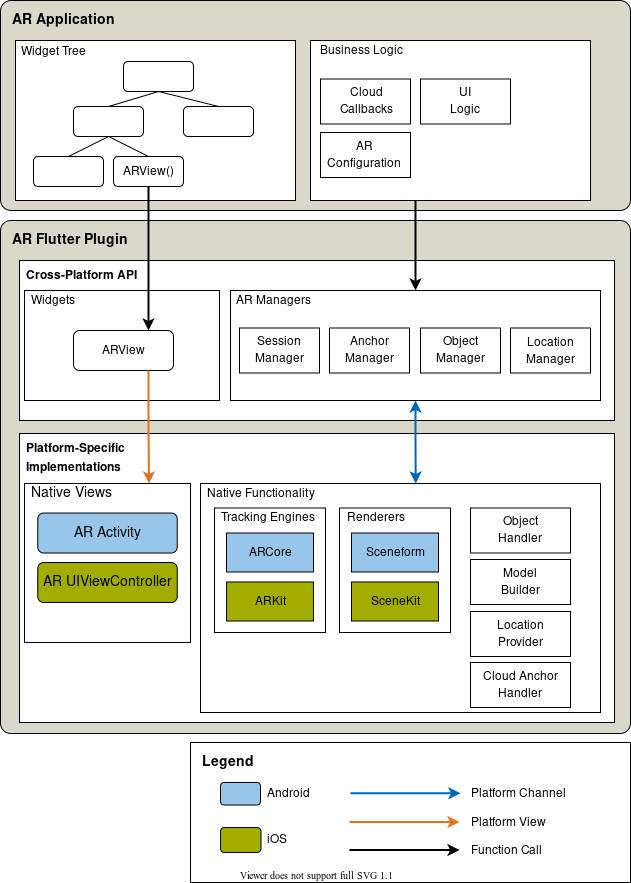
\includegraphics[width=1\textwidth]{ar-flutter-plugin.png}
    \centering
    \caption{Диаграма на архитектурата на ar-flutter-plugin}
    \label{fig:ar-flutter-plugin}
\end{figure}

За съхранение на информацията за мебелите, беше избран JSON формата. Това се дължи главно на лекотата, с която може да се промени кода на приложението, при изпълнение на условието от заданието за разработка на приложнопрогранен интерфейс. JSON също така има преимуществото да използва по-малко пространство при съжраняване на същото количество данни спрямо XML.

По време на разработка, програмата Visual Studio Code беше използвана като развойна среда, за писане на програмния код на мобилното приложение. Основната причина за това беше наличието на добавки към редактора, за поддръжка на всички технологии използвани в проекта (Flutter, TeX, т.н.) Въпреки това, използвани бяха и симулационните компоненти Android Virtual Device (ADV) и Simulator, от Android Studio и XCode съответно, за тестване на приложението. (Фиг. \ref{fig:simulators-screenshot})

\begin{figure}[H]
    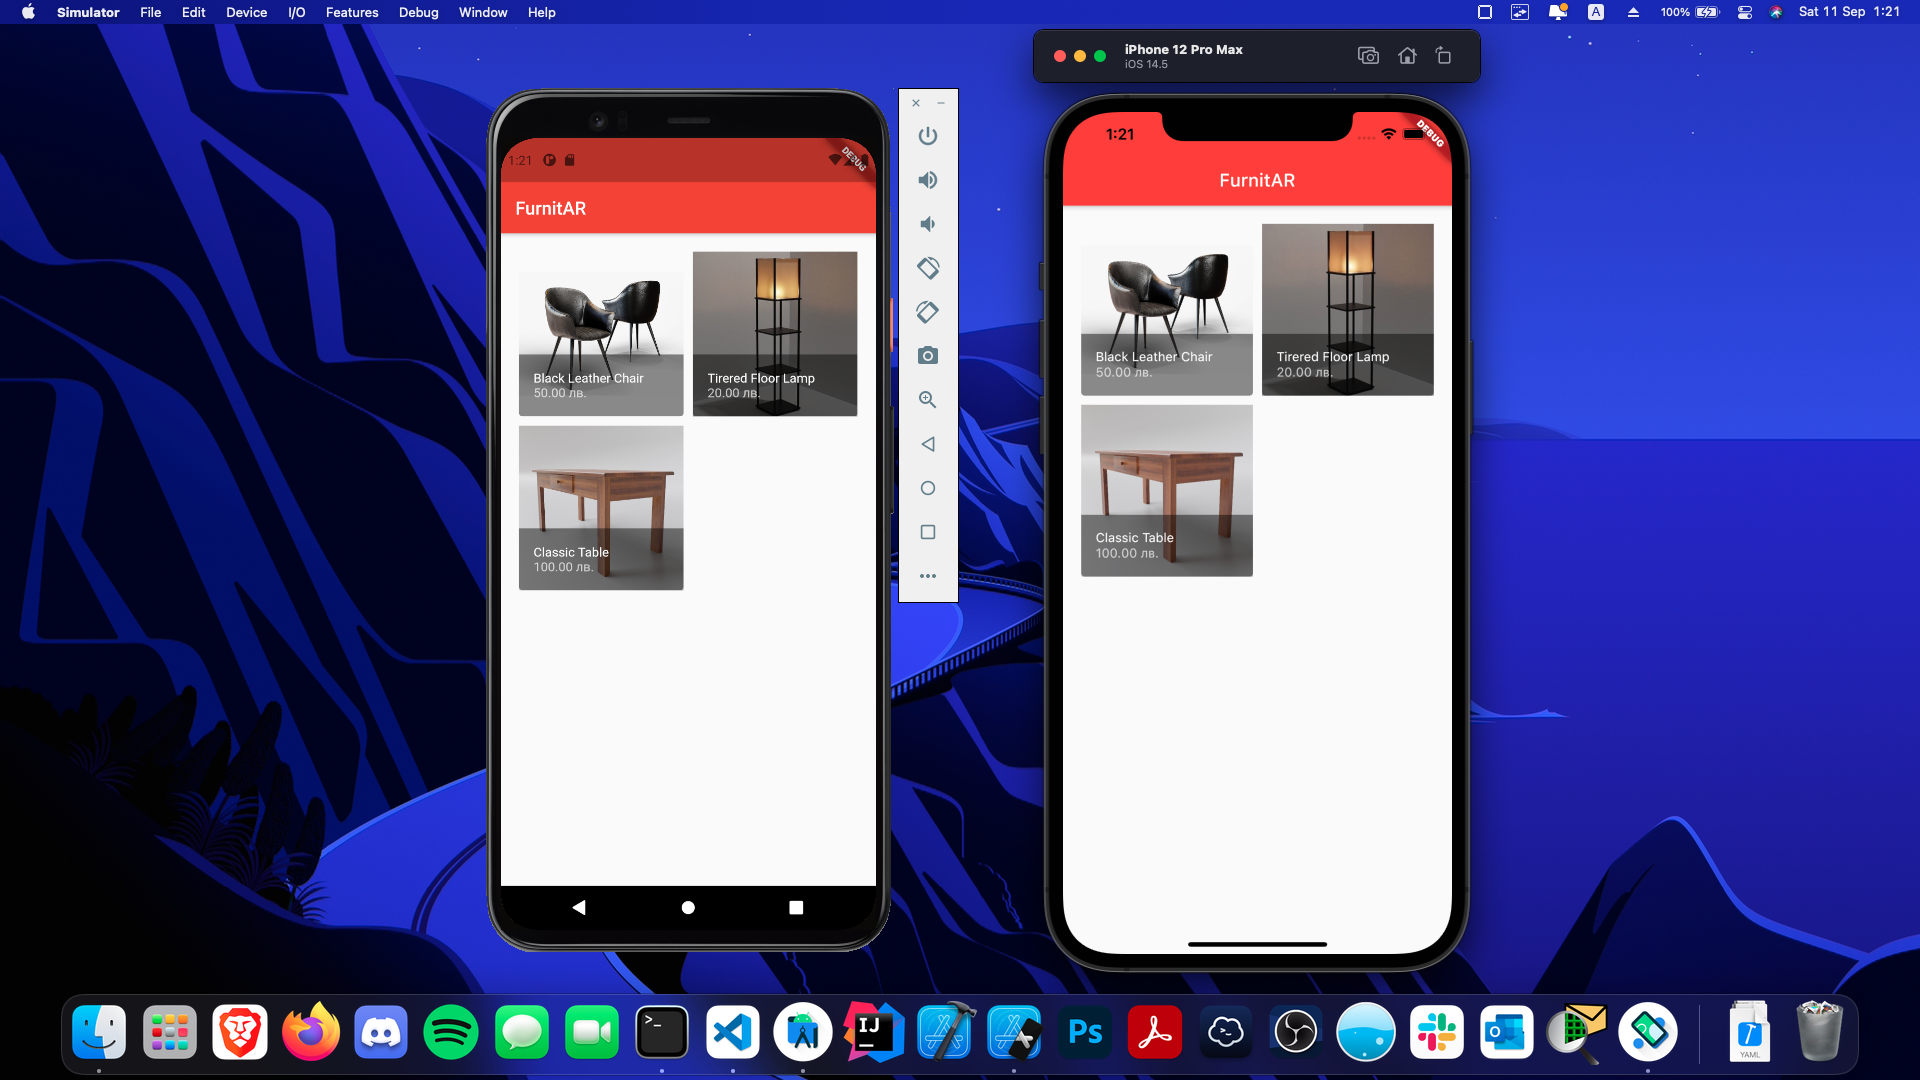
\includegraphics[width=1\textwidth]{simulators-screenshot.png}
    \centering
    \caption{Android Virtual Device (ADV) и XCode Simulator изпълняващи мобилното приложение разглеждано в тази дипломна работа}
    \label{fig:simulators-screenshot}
\end{figure}
